% $Header: /cvsroot/latex-beamer/latex-beamer/solutions/conference-talks/conference-ornate-20min.de.tex,v 1.7 2004/10/07 20:53:08 tantau Exp $

\documentclass[xcolor=dvipsnames]{beamer}

  	\usetheme{Frankfurt}
  	\setbeamertemplate{footline}[frame number]
	\definecolor{RoyalBlue3}{rgb}{0.23,0.37,0.8}
	\definecolor{RoyalBlue4}{rgb}{0.15,0.25,0.54}
	\definecolor{SlateGray4}{rgb}{0.42,0.48,0.54}
	\definecolor{SteelBlue4}{rgb}{0.21,0.39,0.54}
  	\usecolortheme[named=RoyalBlue3]{structure}
	\useinnertheme{circles}  


\usepackage{beamerthemesplit}
\usepackage{color}
\usepackage{graphicx}
\usepackage{epstopdf}
\usepackage{listings}
\usepackage[nomarkers]{pause}
\usepackage{hyperref}
        
\usepackage[german]{babel}
% oder was auch immer

\usepackage[utf8]{inputenc}
% oder was auch immer

\usepackage{times}
\usepackage[T1]{fontenc}


\title[Entwurf] % (optional, nur bei langen Titeln ntig)
{e-puck Conquest}

\subtitle
{Entwurf}

\author[Binder, Bürchner, Freund, Lorenz, Poxrucker, Wilhelm] % (optional, nur bei vielen Autoren)
{SEP - ITS 2010 \\ Max Binder \and Florian Bürchner \and Martin Freund
	\\ Florian Lorenz \and Andreas Poxrucker \and Andreas Wilhelm}
% - Namen mssen in derselben Reihenfolge wie im Papier erscheinen.
% - Der \inst{?} Befehl sollte nur verwendet werden, wenn die Autoren
%   unterschiedlichen Instituten angehren.

\institute[Universität Passau] % (optional, aber oft ntig)
{
  Fakultät für Informatik und Mathematik\\
  Universität Passau}

\AtBeginSubsection[]
{
  \begin{frame}<beamer>
    \frametitle{Inhaltsverzeichnis}
    \tableofcontents[currentsection,currentsubsection]
  \end{frame}
}


% Falls Aufzhlungen immer schrittweise gezeigt werden sollen, kann
% folgendes Kommando benutzt werden:

%\beamerdefaultoverlayspecification{<+->}

\begin{document}

\lstset{language=Java, basicstyle=\footnotesize, tabsize=2}

\begin{frame}
  \titlepage
\end{frame}

\begin{frame}
  \frametitle{Inhaltsverzeichnis}
  \tableofcontents
\end{frame}	

\section{Einleitung}
	\subsection{Einteilung}
		\begin{frame}
			\frametitle{Einteilung des Systementwurfs}
			\begin{figure}[htbp]
				\centering
				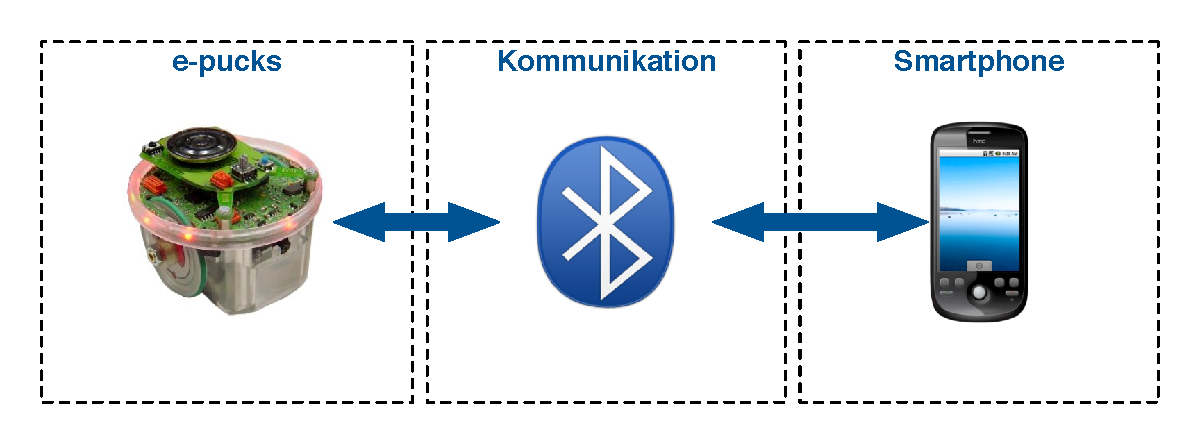
\includegraphics[height=4cm]{images/einteilung.eps}
  			\end{figure}	
		\end{frame}	
	\subsection{Ablauf}
		\begin{frame}
			\frametitle{Sequenzdiagramm}
			\begin{figure}[htbp]
				\centering
				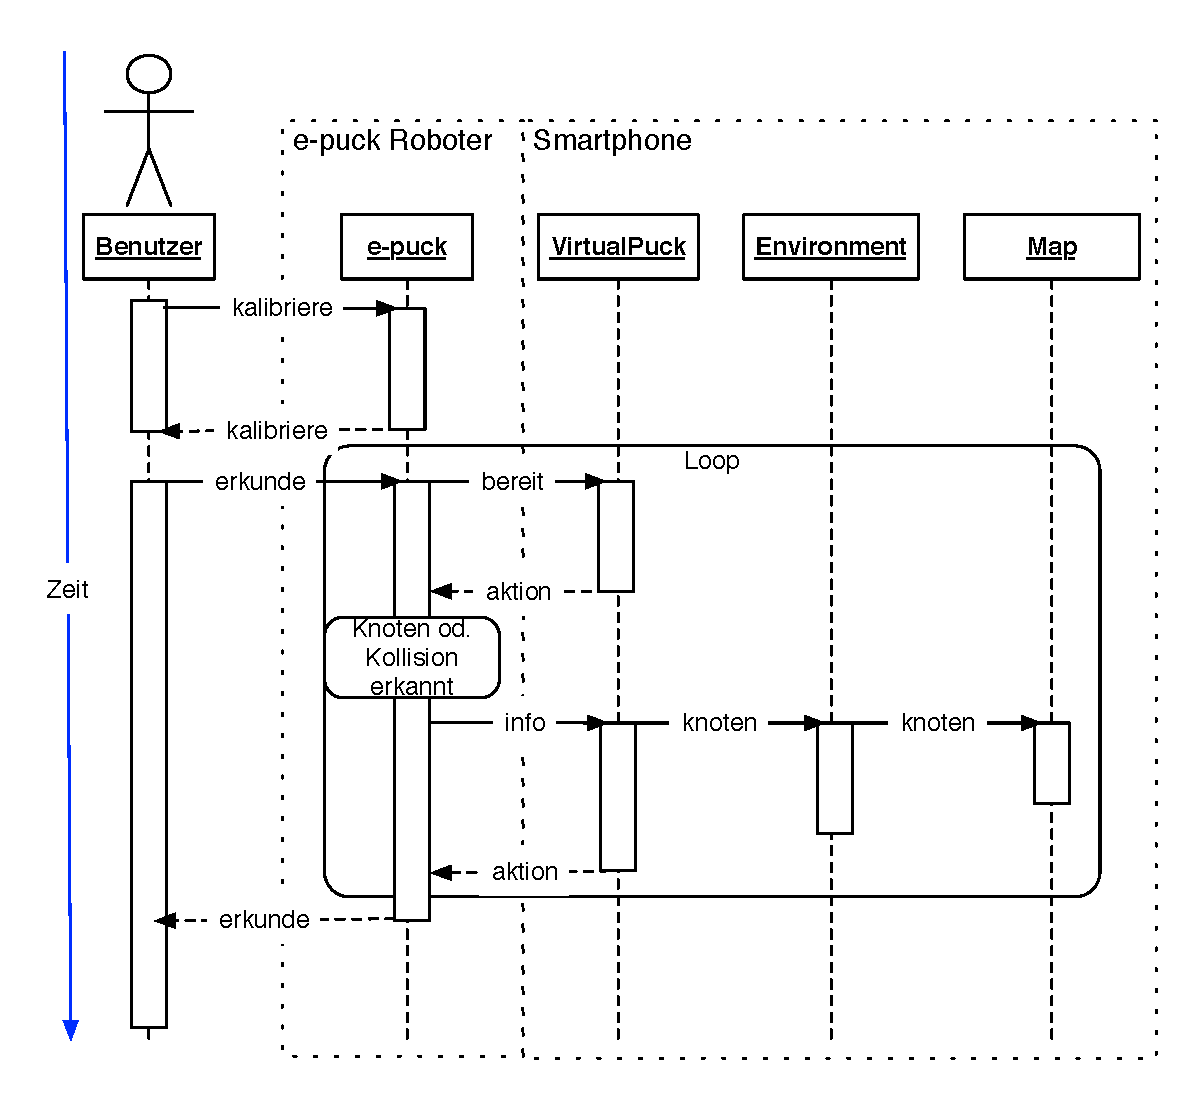
\includegraphics[height=7cm]{images/sequenzdiagramm.eps}
  			\end{figure}	
		\end{frame}	
		
\section[e-puck]{e-puck Roboter}
	\subsection{Komponenten}
		\begin{frame}
			\frametitle{Komponenten des e-puck Roboter}
			\begin{figure}[htbp]
				\centering
				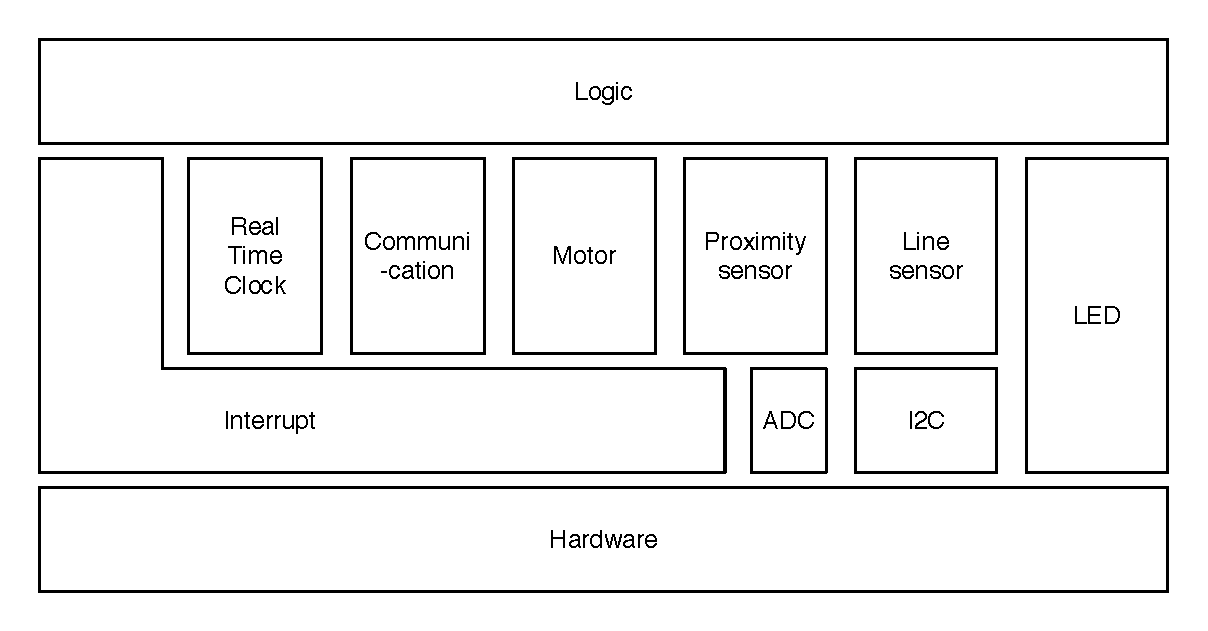
\includegraphics[height=5cm]{images/e-puck_architecture.eps}
  			\end{figure}			
  			\only<2-2>{\textbf{Interrupt}: Ein- Ausschalten von Interrupts
  				\\ \texttt{hal\_int.h, hal\_int.c, hal\_int\_types.h}}
  			\only<3-3>{\textbf{Real Time Clock}: Auslösen von Interrupts; Callbacks
  				\\ \texttt{hal\_rtc.h, hal\_rtc.c, hal\_rtc\_types.h}}
  			\only<4-4>{\textbf{Communication}: Verwaltung von Bluetooth-Verbindungen; Senden, Empfangen
  				\\ \texttt{hal\_uart1.h, hal\_uart1.c, hal\_uart\_types.h}}
  			\only<5-5>{\textbf{Motor}: Funktionen für ``High-Level''-Steuerung der Motoren
  				\\ \texttt{hal\_motor.h, hal\_motor.c, hal\_motor\_types.h}}
  			\only<6-6>{\textbf{ADC}: Funktionen für Analog-Digital-Wandler
  				\\ \texttt{hal\_adc.h, hal\_adc.c, hal\_adc\_types.h}}
  			\only<7-7>{\textbf{I2C}: Funktionen für I2C-Modul
  				\\ \texttt{hal\_i2c.h, hal\_i2c.c}}  
  			\only<8-8>{\textbf{Proximity Sensor}: Initialisierung und Auslesen der IR-Sensoren
  				\\ \texttt{sen\_prox.h, sen\_prox.c, sen\_prox\_types.h}}
  			\only<9-9>{\textbf{Line Sensor}: Auslesen der Sensordaten aus dem I2C-Bus
  				\\ \texttt{sen\_line.h, sen\_line.c, sen\_line\_types.h}}     	
  			\only<10-10>{\textbf{LED}: Initialisierung, Steuerung der LEDs
  				\\ \texttt{hal\_led.h, hal\_led.c}}     	
   			\only<11-11>{\textbf{Logic}: Subsumption...}   										    							
		\end{frame}
	\subsection{Logik}
		\begin{frame}
			\frametitle{Subsumption-Architektur}
			\begin{figure}[htbp]
				\centering
				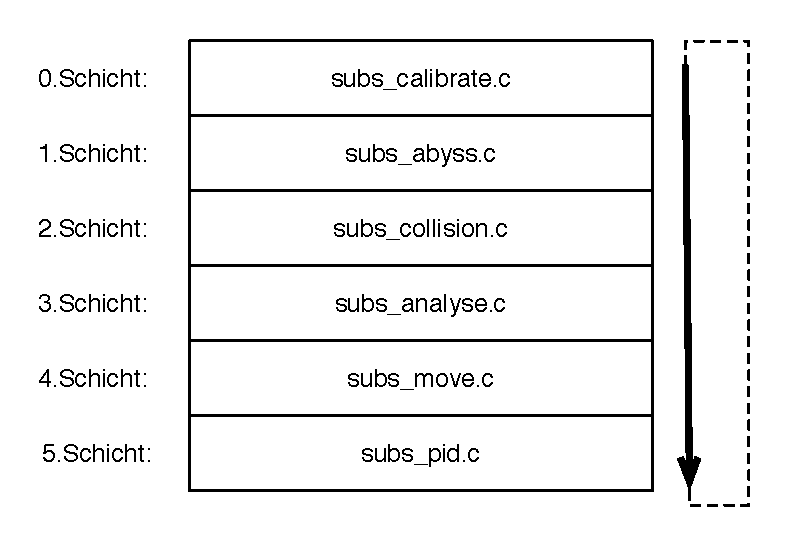
\includegraphics[height=5cm]{images/subsumption.eps}
  			\end{figure}		
  			\only<2-2>{\textbf{0. Schicht}: Kalibriervorgang
  				\\ \texttt{subs\_calibrate.h, subs\_calibrate.c}}
  			\only<3-3>{\textbf{1. Schicht}: Abgrunderkennung
  				\\ \texttt{subs\_abyss.h, subs\_abyss.c}}
  			\only<4-4>{\textbf{2. Schicht}: Kollisionserkennung
  				\\ \texttt{subs\_collision.h, subs\_collision.c}}
  			\only<5-5>{\textbf{3. Schicht}: Knotenanalyse
  				\\ \texttt{subs\_analyse.h, subs\_analyse.c}}
   			\only<6-6>{\textbf{4. Schicht}: Bewegungsmodifikation
  				\\ \texttt{subs\_move.h, subs\_move.c}}
  			\only<7-7>{\textbf{5. Schicht}: Linienvervolgung
  				\\ \texttt{subs\_pid.h, subs\_pid.c}}  				 				
		\end{frame}	

\section[Smartphone]{Android-Anwendung}
	\subsection{Übersicht}
		\begin{frame}
			\frametitle{Klassendiagramm}
			\begin{center}
				\begin{huge}
					Klassendiagramm $\rightarrow$
				\end{huge}
			\end{center}
		\end{frame}	
	\subsection{Komponenten}
		\begin{frame}
			\frametitle{Model-View-Controller}
			\begin{figure}[htbp]
				\centering
				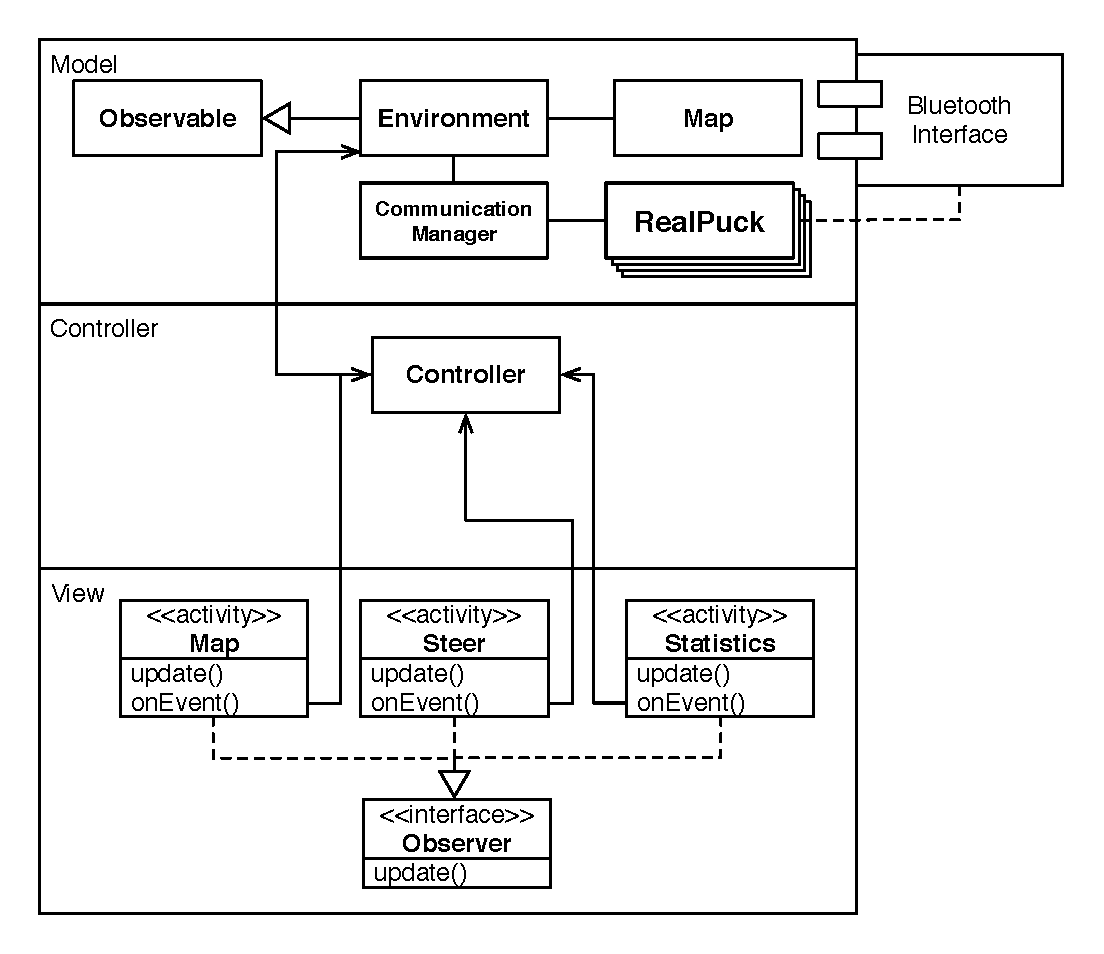
\includegraphics[height=7cm]{images/android_mvc.eps}
  			\end{figure}		
		\end{frame}	
		\begin{frame}
			\frametitle{Environment}
			\begin{figure}[htbp]
				\centering
					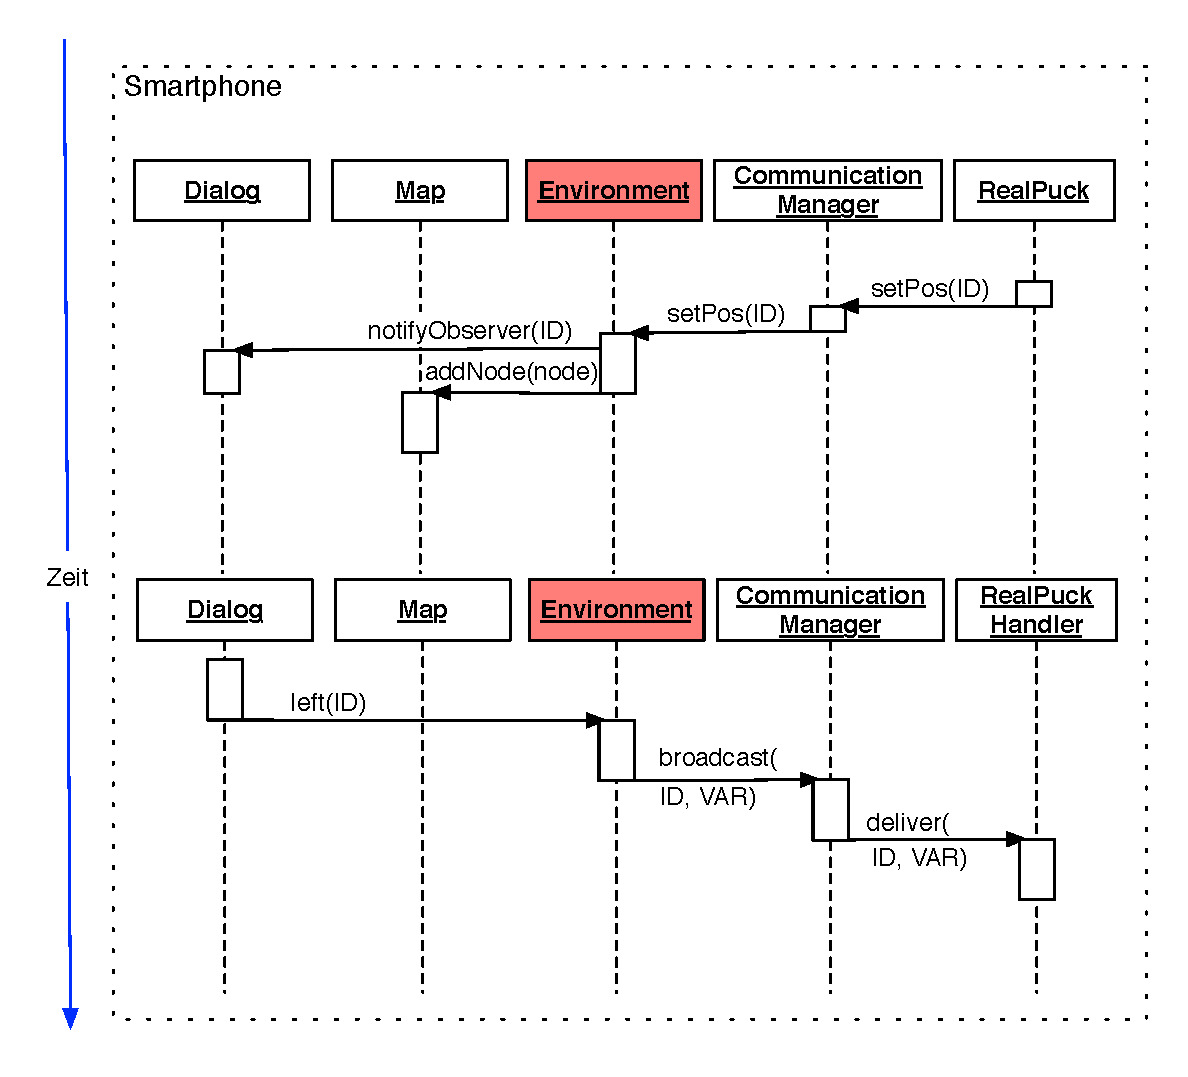
\includegraphics[height=7cm]{images/sequenzdiagramm_environment.eps}
  			\end{figure}		
		\end{frame}	
		\begin{frame}
			\frametitle{Nachrichtenbehandlung (Chain-of-Responsibility)}
			\begin{figure}[htbp]
				\centering
					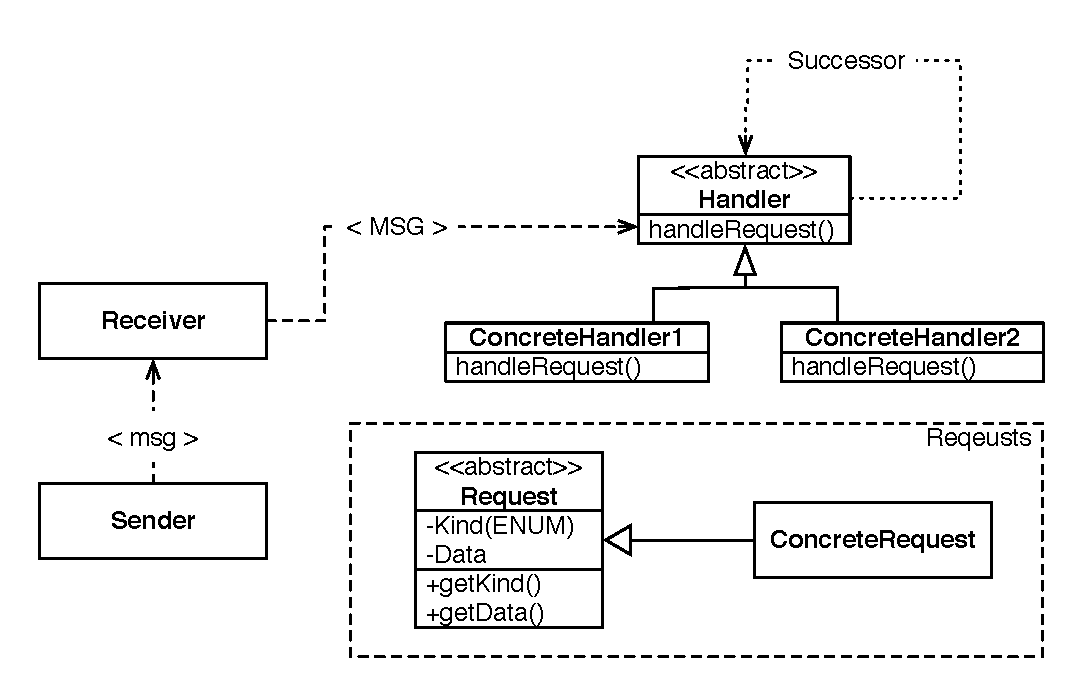
\includegraphics[height=4cm]{images/android_handler.eps}
  			\end{figure}		
		\end{frame}	
		\begin{frame}
			\frametitle{Erkundungsalgorithmus (Schichten-Architektur)}
			\only<1-1>{			
				\begin{figure}[htbp]
					\centering
						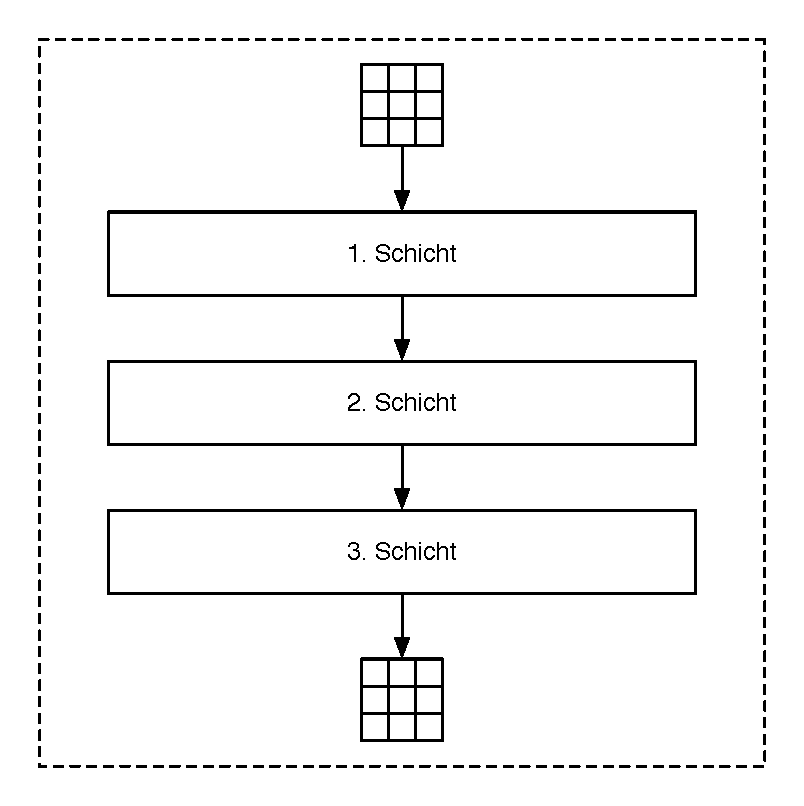
\includegraphics[height=5cm]{images/erkundung_schichten.eps}
  				\end{figure}		
  				}
			\only<2-2>{			
				\begin{figure}[htbp]
					\centering
						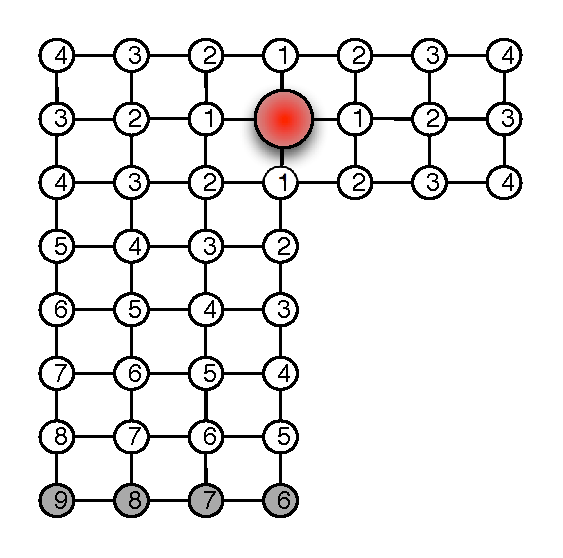
\includegraphics[height=5cm]{images/norm.eps}
  				\end{figure}		
  				}
			\only<3-3>{			
				\begin{figure}[htbp]
					\centering
						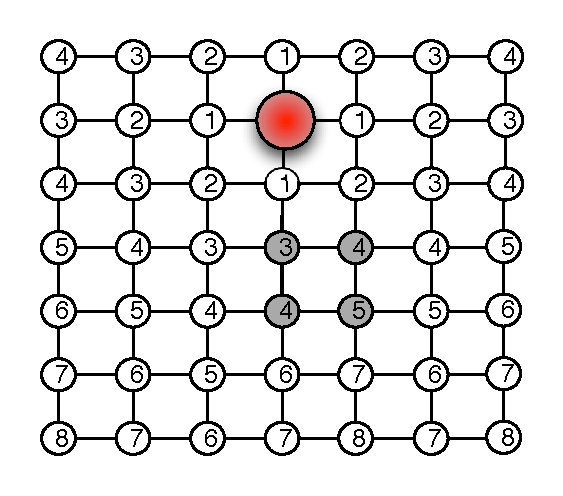
\includegraphics[height=5cm]{images/eingeschlossen.eps}
  				\end{figure}		
  				}  			
			\only<4-4>{			
				\begin{figure}[htbp]
					\centering
						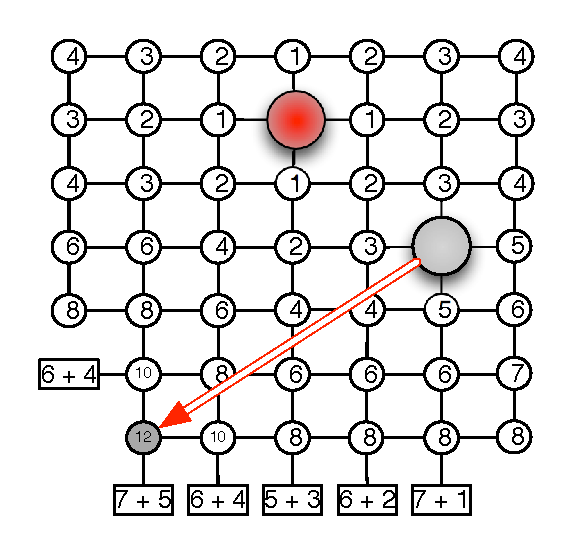
\includegraphics[height=5cm]{images/kooperation.eps}
  				\end{figure}		
  				}  					
		\end{frame}
		\begin{frame}
			\frametitle{Interne Karten-Struktur}
				\begin{figure}[htbp]
					\centering
						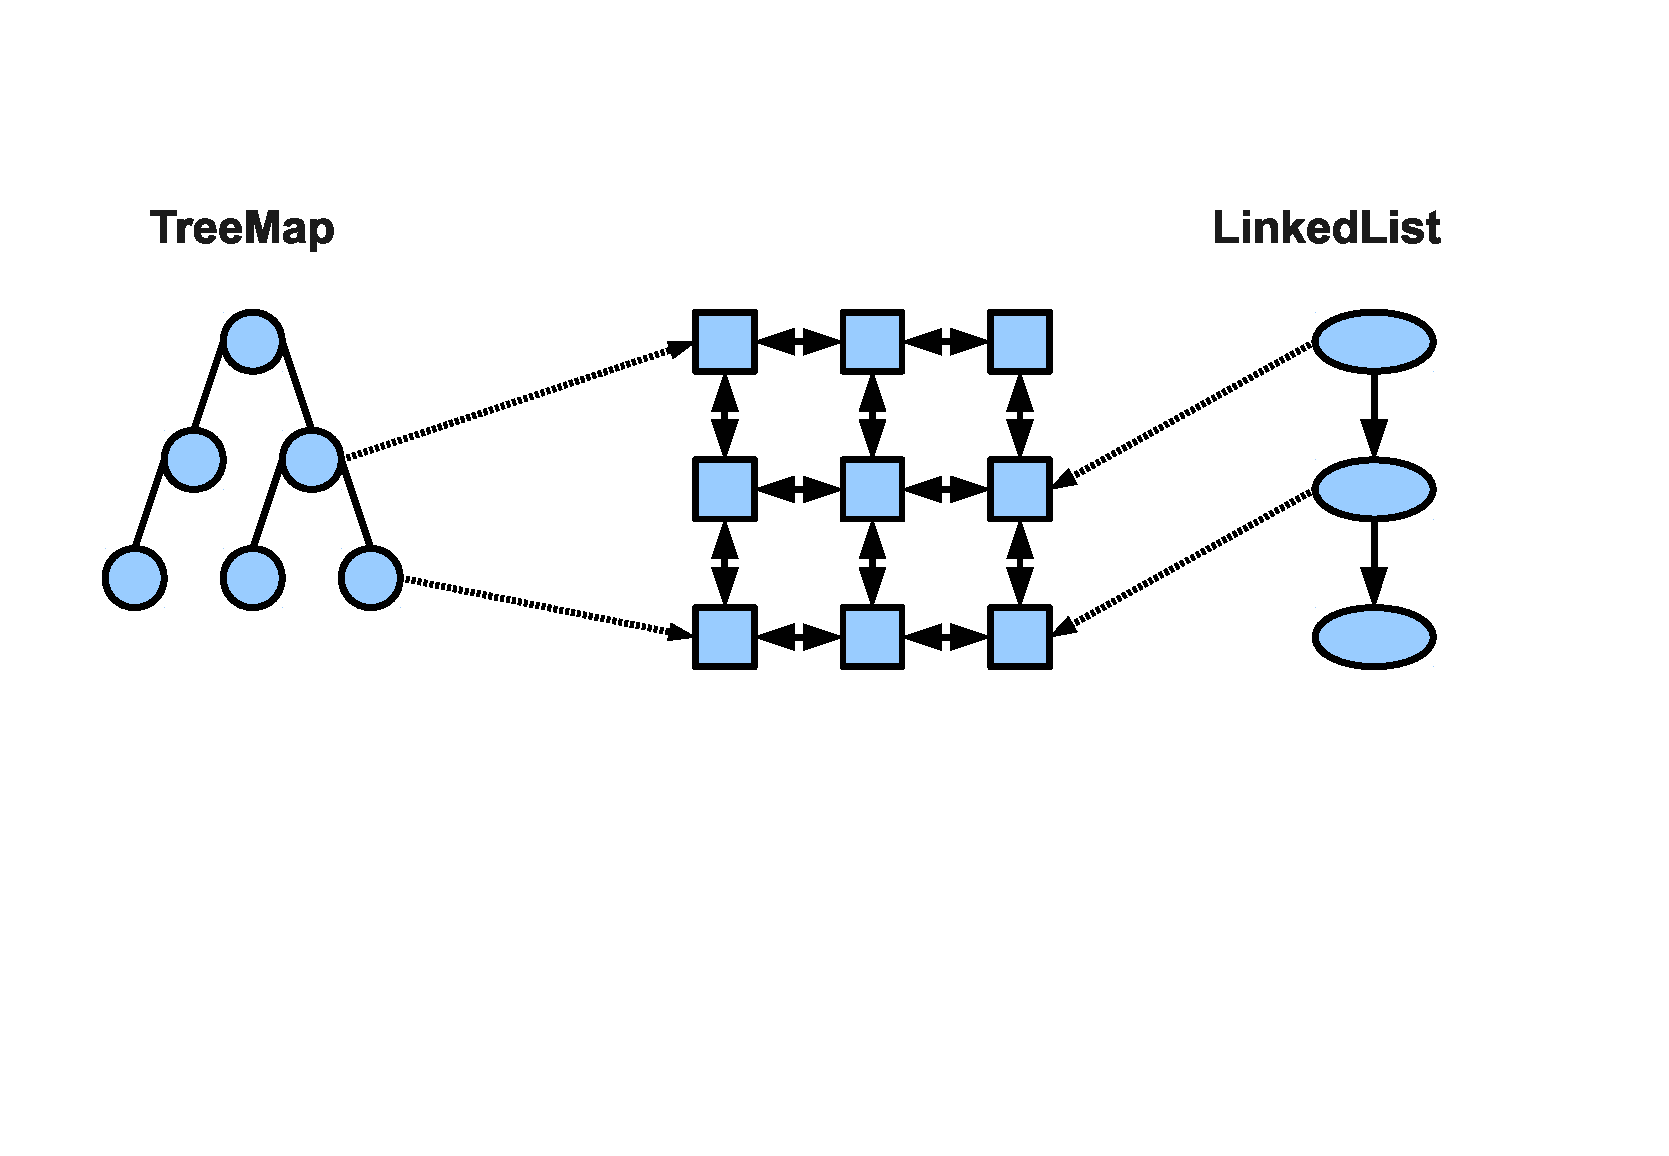
\includegraphics[height=8cm]{images/map.eps}
  				\end{figure}					
		\end{frame}
\section{Ende}
	\begin{frame}
		\begin{center}
			Vielen Dank für die Aufmerksamkeit!
		\end{center}
	\end{frame}
	\begin{frame}
		\frametitle{Sensordaten}
		\begin{figure}[htbp]
			\centering
			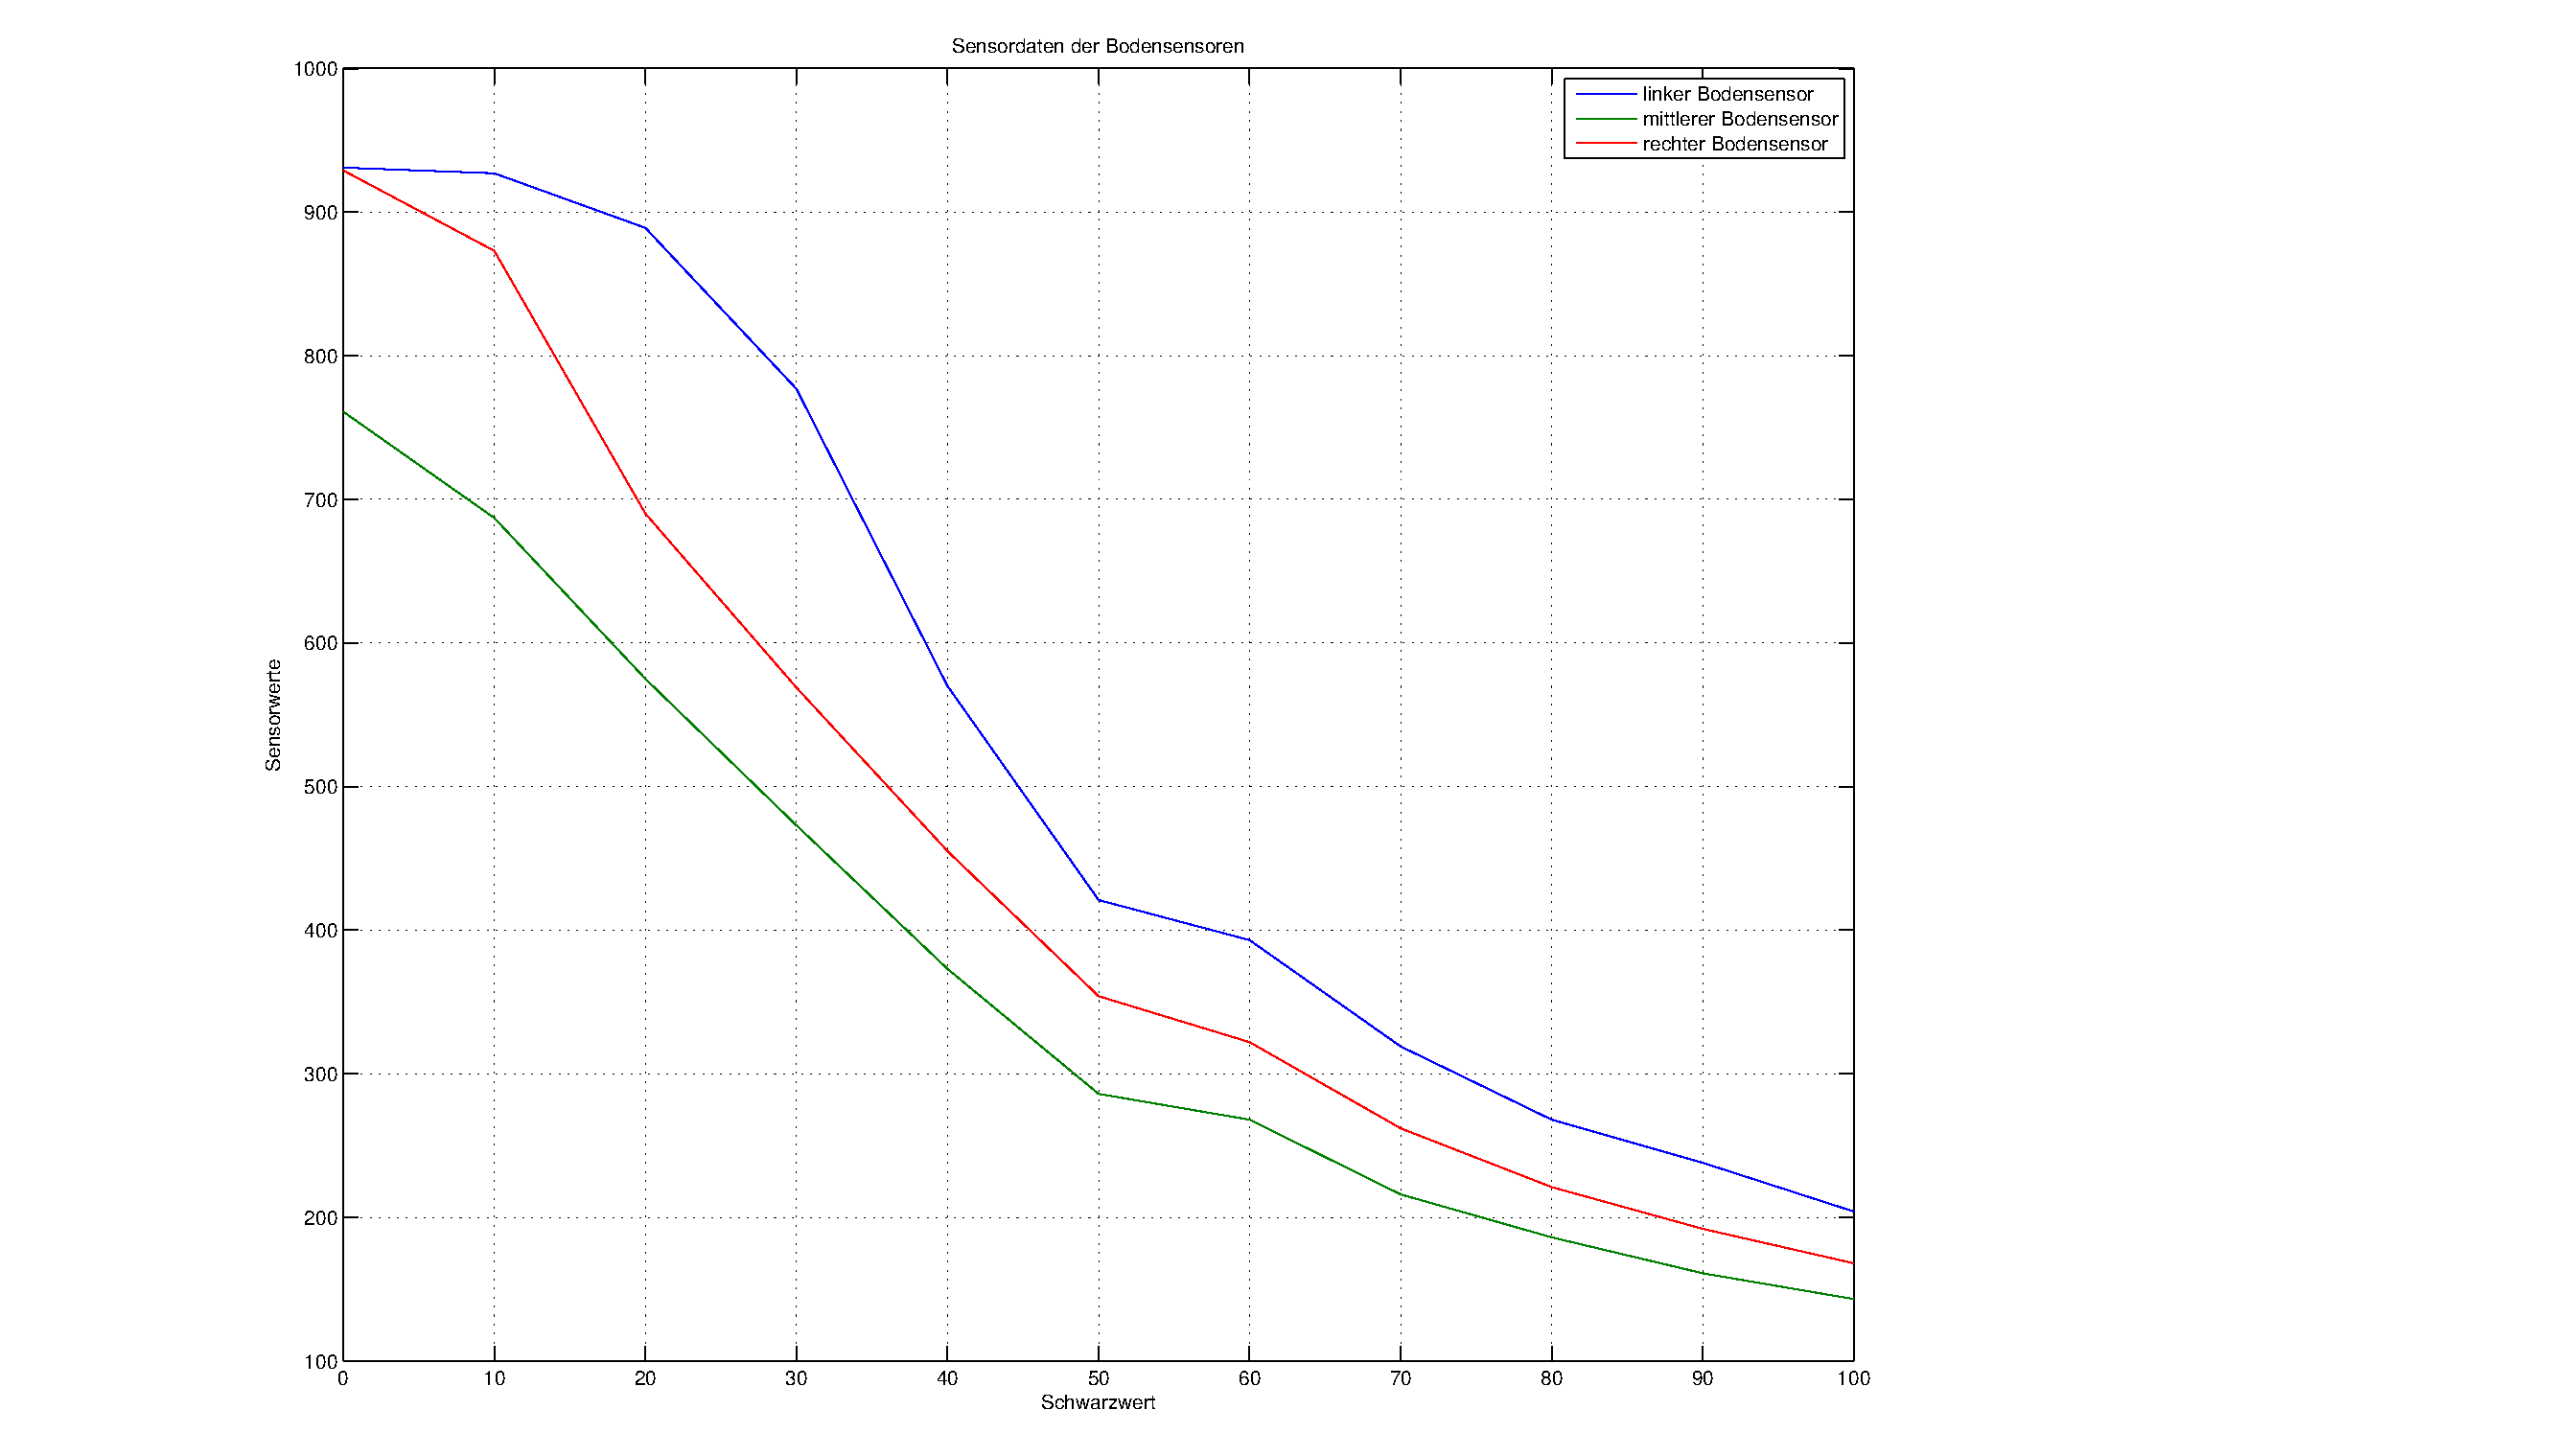
\includegraphics[height=7cm]{images/sensorgrafik.eps}
  		\end{figure}	
	\end{frame}	
		
\end{document}


